\documentclass[border=6pt]{standalone}
\usepackage{tikz}
\usetikzlibrary{arrows.meta,positioning}
\usepackage{helvet}
\renewcommand{\familydefault}{\sfdefault}

\begin{document}
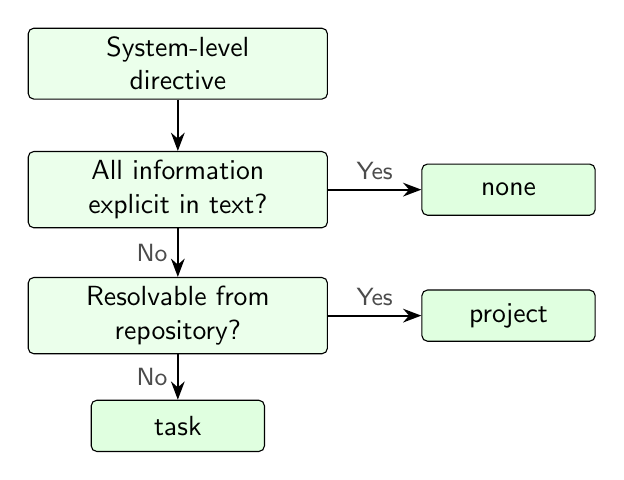
\begin{tikzpicture}[
  >=Stealth,
  decision/.style={draw, rounded corners=2pt, minimum height=0.75cm,
              minimum width=3.8cm, align=center, font=\normalsize,
              fill=green!8},
  outcome/.style={draw, rounded corners=2pt, minimum height=0.65cm,
              minimum width=2.2cm, align=center, font=\normalsize,
              fill=green!12},
  arr/.style={->, thick},
  lbl/.style={font=\small, text=black!70},
]

\node[decision] (start) at (0,5.0) {System-level\\directive};

\node[decision] (cq1) at (0,3.4) {All information\\explicit in text?};
\node[outcome] (none) at (4.2,3.4) {none};

\node[decision] (cq2) at (0,1.8) {Resolvable from\\repository?};
\node[outcome] (proj) at (4.2,1.8) {project};

\node[outcome] (task) at (0,0.4) {task};

\draw[arr] (start) -- (cq1);
\draw[arr] (cq1) -- node[above, lbl] {Yes} (none);
\draw[arr] (cq1) -- node[left, lbl] {No} (cq2);
\draw[arr] (cq2) -- node[above, lbl] {Yes} (proj);
\draw[arr] (cq2) -- node[left, lbl] {No} (task);

\end{tikzpicture}
\end{document}
